%!TEX root = ../dokumentation.tex

\chapter{Hazelcast (Key-Value)} \label{ch:hazelcast}
\chapterauthor{Nick Schroeder, Maxime Fritzsch, Michelle Mersch}

In the following chapter, the Hazelcast database management system will be discussed.
The first part of the chapter will explore the history of Hazelcast,
its different capabilities like its high performance and scalability as well as its fields of application where those capabilities can be
employed to maximum effect.
The second part will then focus on the implementation of Hazelcast, including the requirements, the setup of the cluster and the demonstration of
some of Hazelcast's capabilities by using Hazelcast with some basic relational data to show how it is used.
After this, the third part will then reflect on advantages and disadvantages, explaining how the CAP
theorem can be applied to a Hazelcast cluster and lastly draw a final conclustion on the database as a whole.

\section{Fundamentals} \label{sec:fundamentalsHazelcast}

\subsection{History} \label{subsec:historyHazelcast}

Hazelcast is a distributed In-Memory Data Grid platform, developed for Java. It was created by a company of the same name,
which was founded in 2008 by Talip Ozturk and Fuad Malikov \parencite{DatabaseofDatabases.11032023}. The company's headquarters are
in Palo Alto, California and it also has two European offices in London and Istanbul \parencite{HazelcastContact.03112022}.

After its founding in 2008, the company first released an open-source version of Hazelcast in 2009 and has since been updating it
continously \parencite{DatabaseofDatabases.11032023}. In the time after this first version, Hazelcast has been used by many well known companies,
among them Intel and IBM, the former of which collaborates with Hazelcast on the optimization of in-memory computing solution, while
the latter has a joint initiative with Hazelcast to create and optimize cloud-native applications \parencite{HazelcastPartners.270122}.

\subsection{Capabilities} \label{subsec:capabilitiesHazelcast}

Hazelcast has several features which make it stand out from other solutions to store data, the first of which is how easy it is
to set Hazelcast up and get it running. This is due to the fact that it is self-discovering and self-clustering as Hazelcast's
clusters are formed from different nodes which are all functionally the same, operate in a peer-to-peer fashion and are responsible for
certain data to which they are assigned by the oldest node \parencite{Johns.2015}.

Another important feature of Hazelcast is the fact that it persists data completely in memory, which makes it very fast and efficient.
While this is one of the often cited advantages of Hazelcast, it also has the disadvantage of data being lost if nodes are shut down. To counteract this, Hazelcast usually has copies of data on several different nodes, which
makes the failure of a single node less critical as the data does not get completely lost and can be immediately saved as a backup
in another node. This is depicted in \autoref{fig:hazelcast:example_partitioning}, which shows how the overall data is partitioned into three parts, each of which gets saved by two of the three nodes. Thus, only if more than
one node fails at exactly the same time data can be lost as the standard count of backup nodes is only 1. This number can be increased though if users want to
ensure that their data will not get lost, although this requires more nodes to be operated at the same time \parencite{Johns.2015}.

\begin{figure}[H]
    \centering
    \caption[Example for partitioning in Hazelcast]{Example for partitioning in Hazelcast, \parencite{Johns.2015}} \label{fig:hazelcast:example_partitioning}
    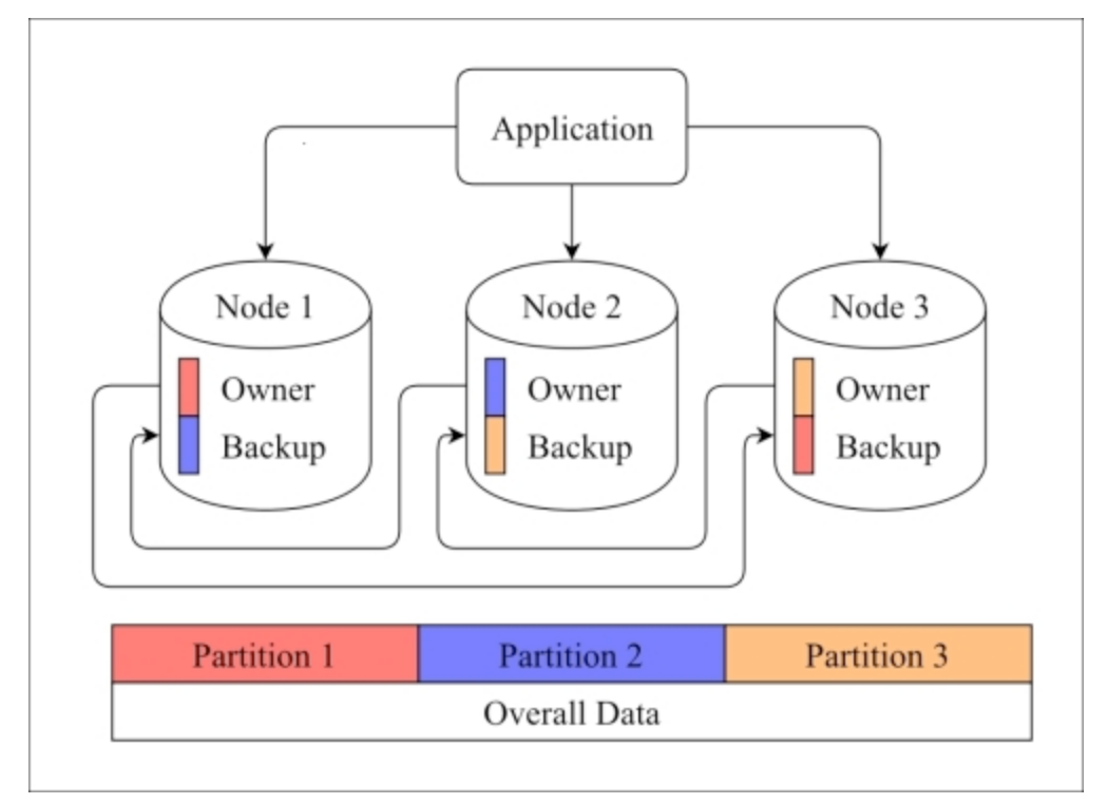
\includegraphics[width=0.7\textwidth]{images/hazelcast_partitioning.png}
\end{figure}

Another capability of Hazelcast is its diverse offering of ways to store data, including standard utility collections like lists, sets and queues as well as Maps, which enable users to save data as key-value pairs. Additionally to those basic Maps, Hazelcast also offers
specialized collections like Multi-Maps, which allow for multiple values per key \parencite{Johns.2015}.

\subsection{Fields of Application} \label{subsec:fieldsOfApplicationHazelcast}

Hazelcast can be used in numerous different ways, one of which would be to hold data for user sessions, an application that makes sense due to its nature
of persisting data only in memory and it thus being well suited for working with temporary data. Furthermore, another application of Hazelcast is
running it together with a data store that persists data long term, leading to an increased capacity. Overall Hazelcast is in general well
suited for applications which require a high performance and elastic scalability as those are both requirements Hazelcast fulfills due to it saving data in memory and
its automatic clustering \parencite{Johns.2015}.

\section{Implementation} \label{sec:implementationHazelcast}

In the second section of this chapter, a hazelcast cluster will be set up, including a cluster management
instance. Then, some capabilities are demonstrated using a simple dataset of relational data, highlighting
the differences between it and a traditional SQL database.

\subsection{Requirements} \label{subsec:requirementsHazelcast}

To deploy a hazelcast cluster on a local machine, \textcite{Hazelcast.Docker.Hazelcast, Hazelcast.Docker.ManagementCenter} is used, utilising the existing images,
\enquote{hazelcast/hazelcast}  and \enquote{hazelcast/management-center}.
Following the official documentation, two member instances are set up alongside a single cluster manager,
simulating a cluster environment. The cluster manager is then accessible via port 8080, providing status
information about the cluster members. To fully interact with the cluster, it is necessary to install a
client. \textcite{Hazelcast.Clients} supports a handful of open-source APIs in multiple programming languages.
Within the scope of this document, the python client is
used in the following sections to demonstrate data import and access. The client can be installed with pip
or any preferred python package manager.

\subsection{Data Import} \label{subsec:dataImportHazelcast}

Once everything is ready, one can import the data into the hazelcast cluster. The following figure displays
a simple relational data model, which will serve as an example.

\begin{figure}[H]
    \centering
    \caption{Hazelcast Implementation Example (Custom Graphic)} \label{fig:hazelcast.implementation.tables}
    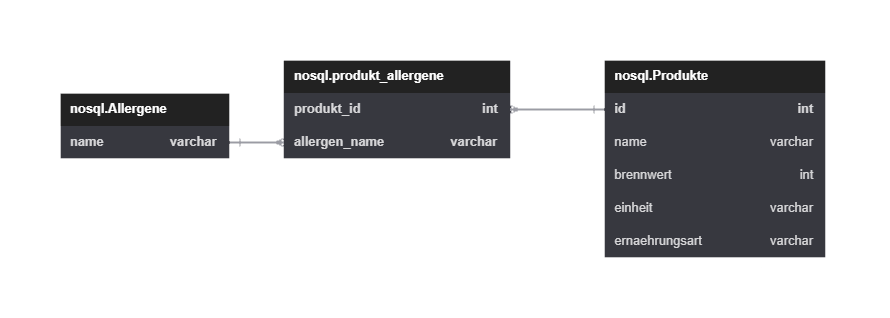
\includegraphics[width=\textwidth]{images/hazelcast.implementation.tables.png}
\end{figure}

The table on the left contains only one attribute, the primary key. Depending on the requirements,
there are two possible data structures to represent this table in a key-value store.
The \textcite{Hazelcast.DataStructure.Set}, similar to
the built-in python data type, is a list of elements. It disallows duplicates, imitating the primary
key constraint of a relational database.
However, as a non-partitioned data structure,
all elements of a single set are kept on one cluster member. Thus, a Set should not be used with a great number of elements.
The second structure is the \textcite{Hazelcast.DataStructure.Map}. It is a distributed structure and split between single members.
Additionally, based on the Java Map, its ordinary time
complexity is quite efficient, as explained by \textcite{Hazelcast.Java.Map}
Therefore, a Map is used to represent the \enquote{Allergene} table.
However, a synthetic key is required to insert and access values.
An incremental integer could provide this, as shown in the figure below.


\begin{figure}[H]
    \centering
    \caption{Hazelcast Allergens Map} \label{fig:hazelcast.allergens.map}
    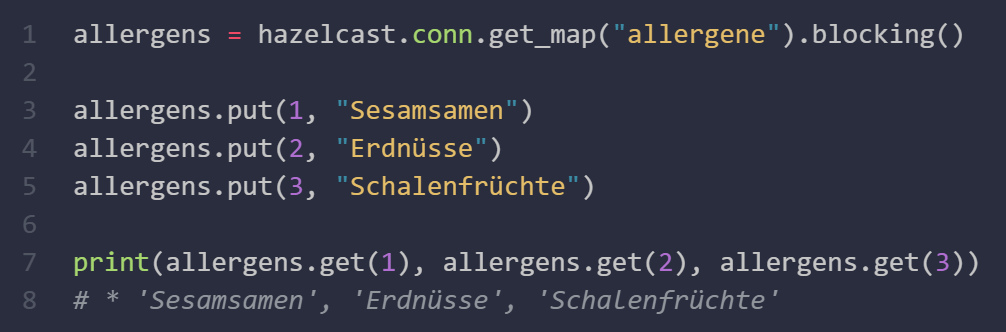
\includegraphics[width=\textwidth]{images/hazelcast.allergens.map.png}
\end{figure}

Not only can a Map store primitive values such as integers or strings, but also more complex ones, for
example, JSON Objects. The python client can readily encode JSON Objects and store them on the cluster,
which will be used for the \enquote{Products} table.
\parencite{Hazelcast.PythonClient.HazelcastJsonValue}

\begin{figure}[H]
    \centering
    \caption{Hazelcast Products Map} \label{fig:hazelcast.products.map}
    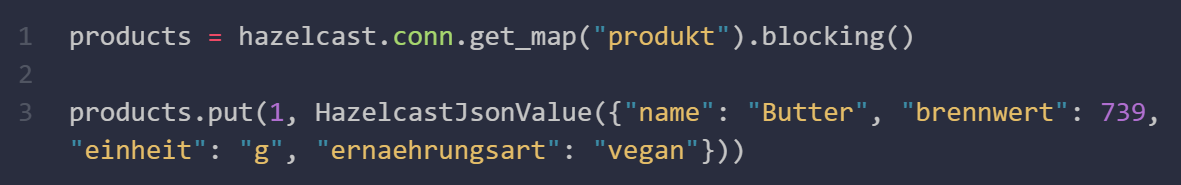
\includegraphics[width=\textwidth]{images/hazelcast.products.map.png}
\end{figure}

Nevertheless, to insert new values, an application has to keep track of the current integer key and check
for duplicates since a Map does not enforce unique values. Additionally, as Maps are meant to be flexible,
they do not enforce type constraints. Therefore, data validation should be handled by an application before
manipulating data on the cluster.
The last table, \enquote{produkt\_allergene},
represents a many-to-many relation and therefore holds entries with the
same \enquote{produkt\_id} but different \enquote{allergen\_name}, as one product may contain multiple allergens.
Using a Map and manually encoding a list of allergens similar to that shown in \autoref{fig:hazelcast.allergens.map}
would be possible. Since all allergens are known at the time of creation, the
list is not updated frequently. However, if the list is regularly updated or contains many elements, it
would be required to load all entries on the application side, manipulate it and overwrite the old version
on the hazelcast cluster.
Thus, Hazelcast supports \textcite{Hazelcast.DataStructure.MultiMap}, another distributed key-value data structure that is able to hold
multiple values per key, preventing duplicates for one key.
An example of inserting elements into a MultiMap is shown below.

\begin{figure}[H]
    \centering
    \caption{Hazelcast Product Allergens MultiMap} \label{fig:hazelcast.product_allergens.1.multimap}
    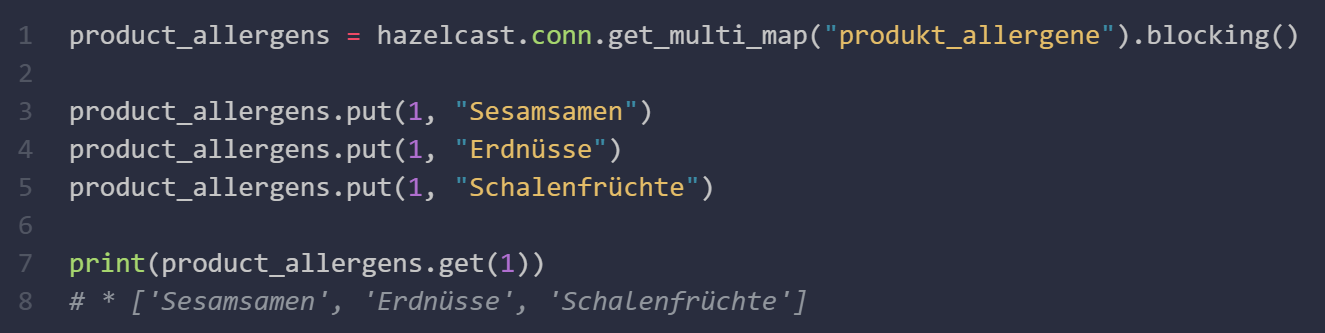
\includegraphics[width=\textwidth]{images/hazelcast.product_allergens.multimap.1.png}
\end{figure}

\subsection{Data Access} \label{subsec:dataAccessHazelcast}

When it comes to accessing data, problems may occur if the key of a particular entry is unknown or one wants
to query an entire map for multiple key-value pairs that fulfil certain conditions. For such use cases,
hazelcast offers \enquote{Predicates}, methods similar to SQL to query a cluster \parencite{Hazelcast.Predicates}.
A small sample of their capabilities is shown below.

\begin{figure}[H]
    \centering
    \caption{Hazelcast Predicates} \label{fig:hazelcast.predicates}
    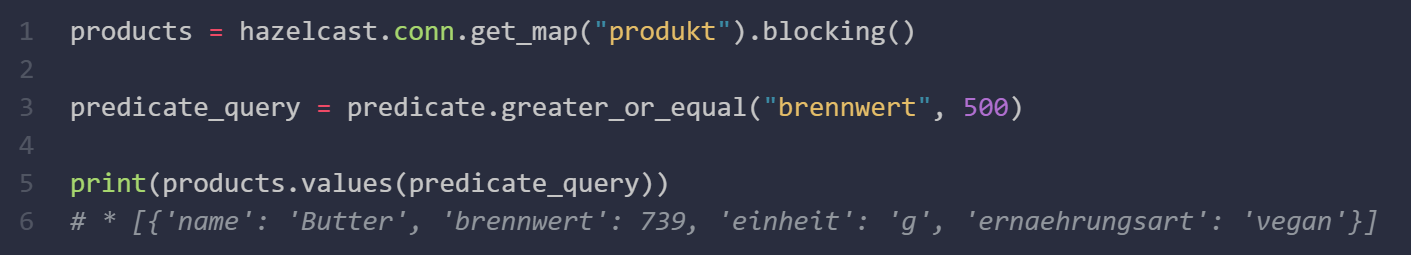
\includegraphics[width=\textwidth]{images/hazelcast.predicates.png}
\end{figure}

Nonetheless, referring back to the \enquote{produkt\_allergene} table, one might not only want to know all
allergens of one particular product but also all products which contain one particular allergen.
Depending on the use case, it may therefore be useful to create copies of maps and rearrange them
to simplify access to data from multiple perspectives. As shown in
\autoref{fig:hazelcast.product_allergens.2.multimap}, a second Map is created using the allergenes as key
to access all products that contain a particular allergen.

\begin{figure}[H]
    \centering
    \caption{Hazelcast Allergens Product MultiMap} \label{fig:hazelcast.product_allergens.2.multimap}
    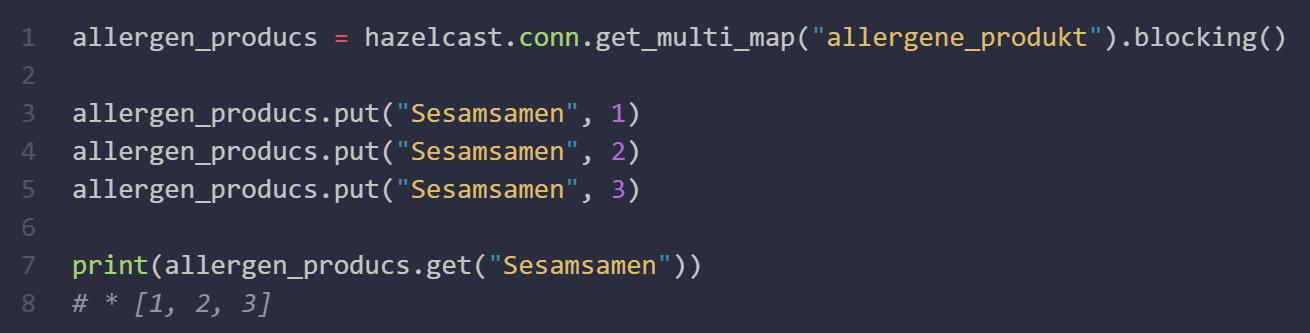
\includegraphics[width=\textwidth]{images/hazelcast.product_allergens.multimap.2.png}
\end{figure}

\section{Reflection} \label{sec:reflectionHazelcast}

\subsection{Advantages \& Disadvantages} \label{subsec:advantagesDisadvantagesHazelcast}

One of the advantages of Hazelcast is the high availability. Members discover each other automatically and form a cluster.
After the cluster is formed, members communicate with each other.  Every cluster member can become inaccessible because of network
failure or other events. The other cluster members cooperatively diagnose that state and immediately take over the responsibility of the failed member. Hazelcast can restore the data and provides continuous availability.

It also offers distributed implementation of standard collections. These implementations include Maps, Lists, Sets and others. Also,
it has a broadcast messaging system that works with publish and subscribe models. This communication works with real time at high speed.
Hazelcasts SQL service lets you query static and streaming data. Static data can be loaded from sources to transform and analyze it.
Furthermore it is possible to load and query real time streaming data as it is being generated.
Another marked feature is that it has no dependency on disk storage. It keeps all its operational state in the dynamic random access
memory of the cluster. Hazelcast can conduct really quick readings and updates and save everything in memory.
Hazelcast is also a Java application with no external dependencies which offers the same APIs and interfaces as the Java util package.

But there are also some disadvantages of Hazelcast. The memory sharing system can be difficult to implement and understand in the
beginning. Working with the Hazelcast database is something one has to get used to. Once one has understood how everything works, it is easy to use.
Another disadvantage is running Hazelcast in a virtual environment. This could create a potential time adjustment and difference
between the CPU and the virtual environment´s adjusted system clock. When the differences go beyond certain ties, Hazelcast usually
initiates a disconnect to solve this problem \parencite{Oguejiofor.05.10.2022}.

\subsection{CAP Theorem} \label{subsec:capTheoremHazelcast}

The CAP Theorem is a fundamental concept in distributed system. It explains, that it is impossible for
this kind of system to provide all three of the following properties from \textcite[23]{Brewer.2012}:

\begin{enumerate}
    \item Consistency: Consistency of the saved data. All clients are able to get the same data at the same time. Every read operation of the systems should return the most recently changed data.
    \item Availability: Every not failing node should return a response for all read and write requests in a reasonable time frame.
    \item Partition tolerance: The system continues to work even when the network partitions.
\end{enumerate}

According to this theorem, a distributed system can only provide two of these guarantees at the same
time. System designers have to choose which two of these properties they want to prioritize for their
application. The theorem has implications for a wide variety of distributed systems, including databases,
storage systems and others \parencite[1]{Brewer.2017}.
Hazelcast as an AP system delivers availability and partition tolerance at the expense of consistency.
The data of all members will remain available even if there is a communication breakdown.
However, some members affected by the partition might return older versions of the data than others.
After a partition has been resolved, Hazelcast syncs all members to resolve any inconsistencies in the
system. The data structures exposed by Hazelcast are all AP data structures.
But there is also a function  that provides CP structures, which are built on the raft consensus algorithm.
As a CP system, Hazelcast  delivers consistency and partition tolerance at the expense of availability.
Whenever a partition occurs between existing members, Hazelcast makes the non-consistent member
unavailable until the partition is resolved \parencite{Hazelcast.05.04.2023}.

\subsection{Conclusion} \label{subsec:conclusionHazelcast}

In conclusion, Hazelcast is a good choice for a distributed system. It is a fast and easy-to-use database as well as
flexible and great at storing time series or session data. However, it is difficult to enforce data validation, thus,
not suitable for all use cases. Hazelcast is used best as a secondary database in combination with relational or other types of databases on top.

